\documentclass[12pt,fleqn]{article}
\usepackage[margin=0.5in]{geometry}
\usepackage{amsmath, amssymb}
\usepackage{enumitem}
\usepackage{pdfpages}
\usepackage{tikz}
\usetikzlibrary{trees}

\setlength{\mathindent}{0pt}
\allowdisplaybreaks

\title{COMP 4190 Assignment 2 Answer}
\author{Fidelio Ciandy, 7934456}
\date{}

\begin{document}
\maketitle

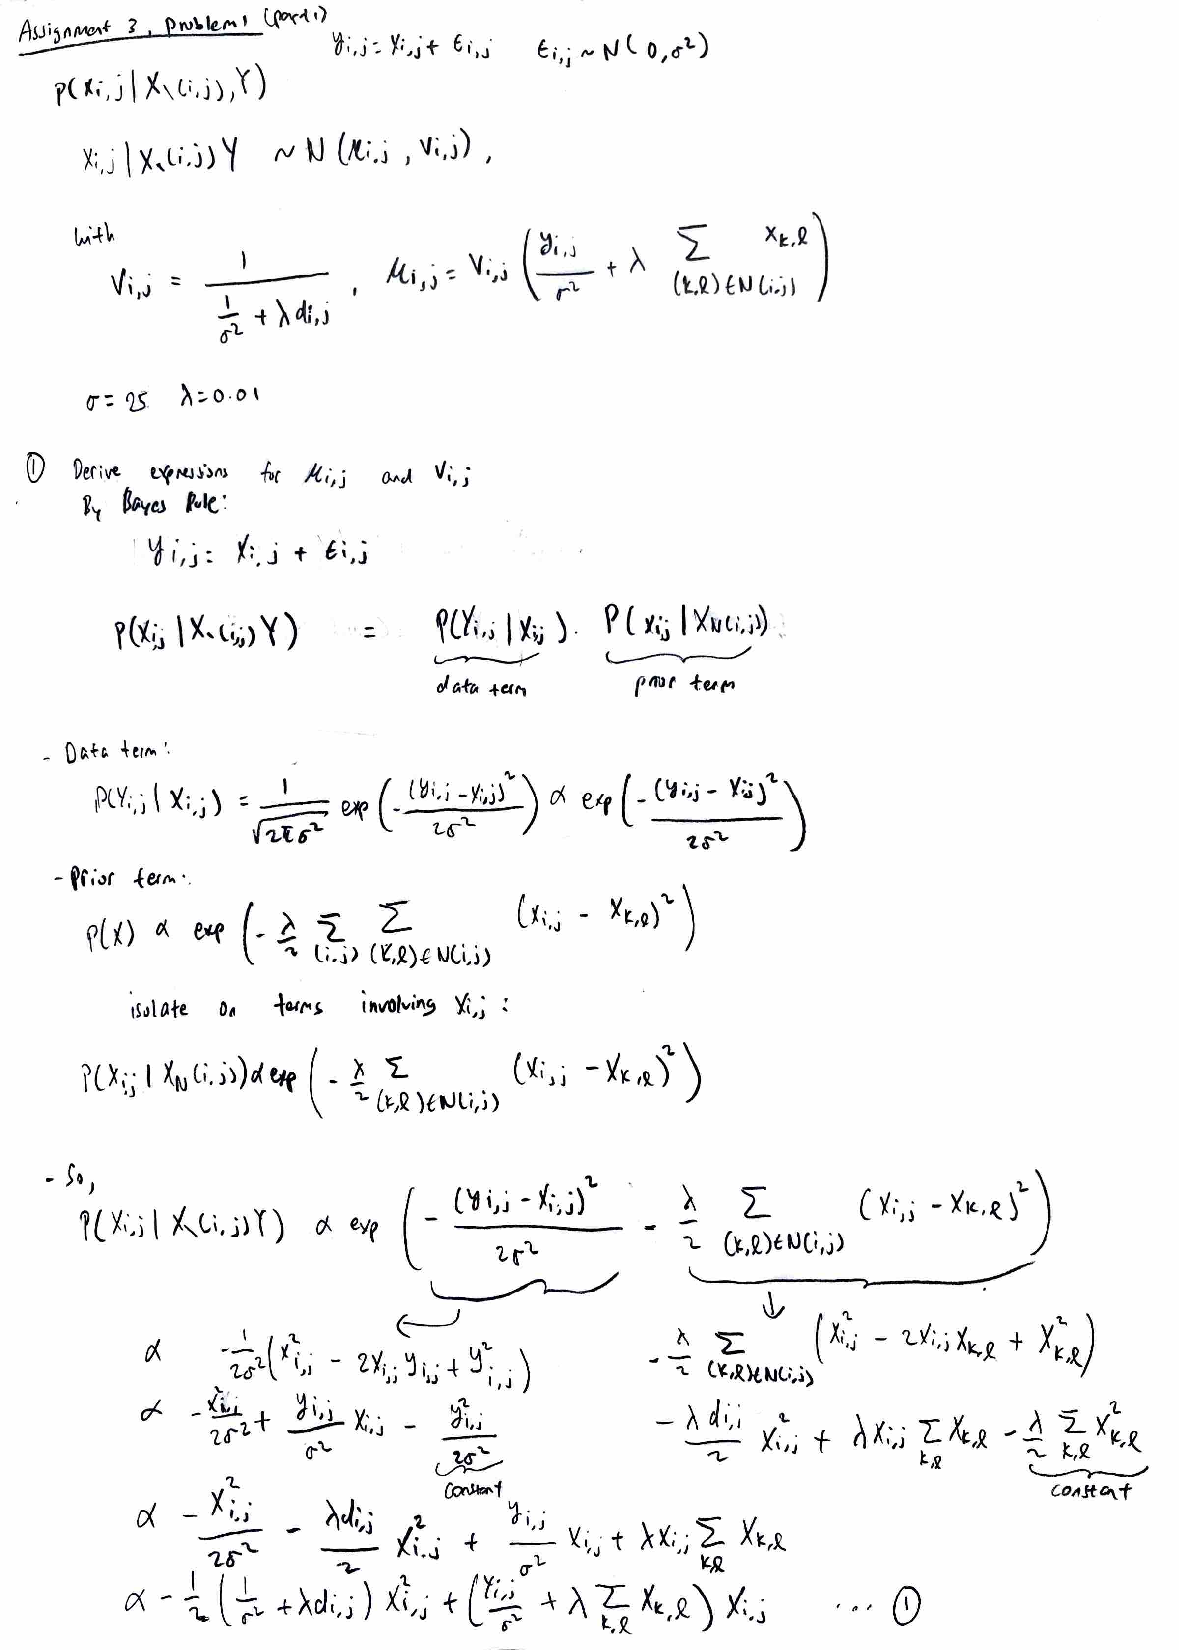
\includepdf[pages={1,2}]{A3-report-writing.pdf}

\section*{Problem 1, Question 2 and 3}
Problem1.py consist of 2 different functions

\begin{itemize}
  \item \textbf{noisy\_image\_Y}
  \begin{itemize}
    \item This function takes in a file path
    \item Uses the numpy library to convert that text file that consist of a 2d array into a noisy image
  \end{itemize}

  \item \textbf{gibbs\_sampling}
  \begin{itemize}
    \item Gibbs sampling for image denoising
    \item First, copy the noisy image as the starting point
    \item Then, calculate the neighbors around each pixel
    \item For each pixel using scanline order, sample a new value based on its neighbors and the original noisy value
    \item Repeat this for many sweeps, then average the results to get the denoised image
  \end{itemize}
\end{itemize}

\includepdf[pages={3-}]{A3-report-writing.pdf}

\end{document}